\documentclass[11pt]{article}
\usepackage[a4paper, left=3 cm,
right=3 cm,
top=3 cm,
bottom=2cm]{geometry}

\usepackage{setspace}

\usepackage{abstract}
\usepackage{booktabs}
\usepackage{comment}
\usepackage{graphicx}
\usepackage{import}
\usepackage[hidelinks]{hyperref}
\usepackage{etoolbox}
\AtBeginEnvironment{tabular}{\footnotesize}

\usepackage[font=footnotesize,labelfont={it}]{caption}



%Bibisetup
\usepackage[round]{natbib}
%\usepackage{cite}
\bibliographystyle{plainnat}
\usepackage{float}
\floatstyle{boxed}



\begin{comment}
\import{"../output/BE/table/"}{"aicc_df.tex"}
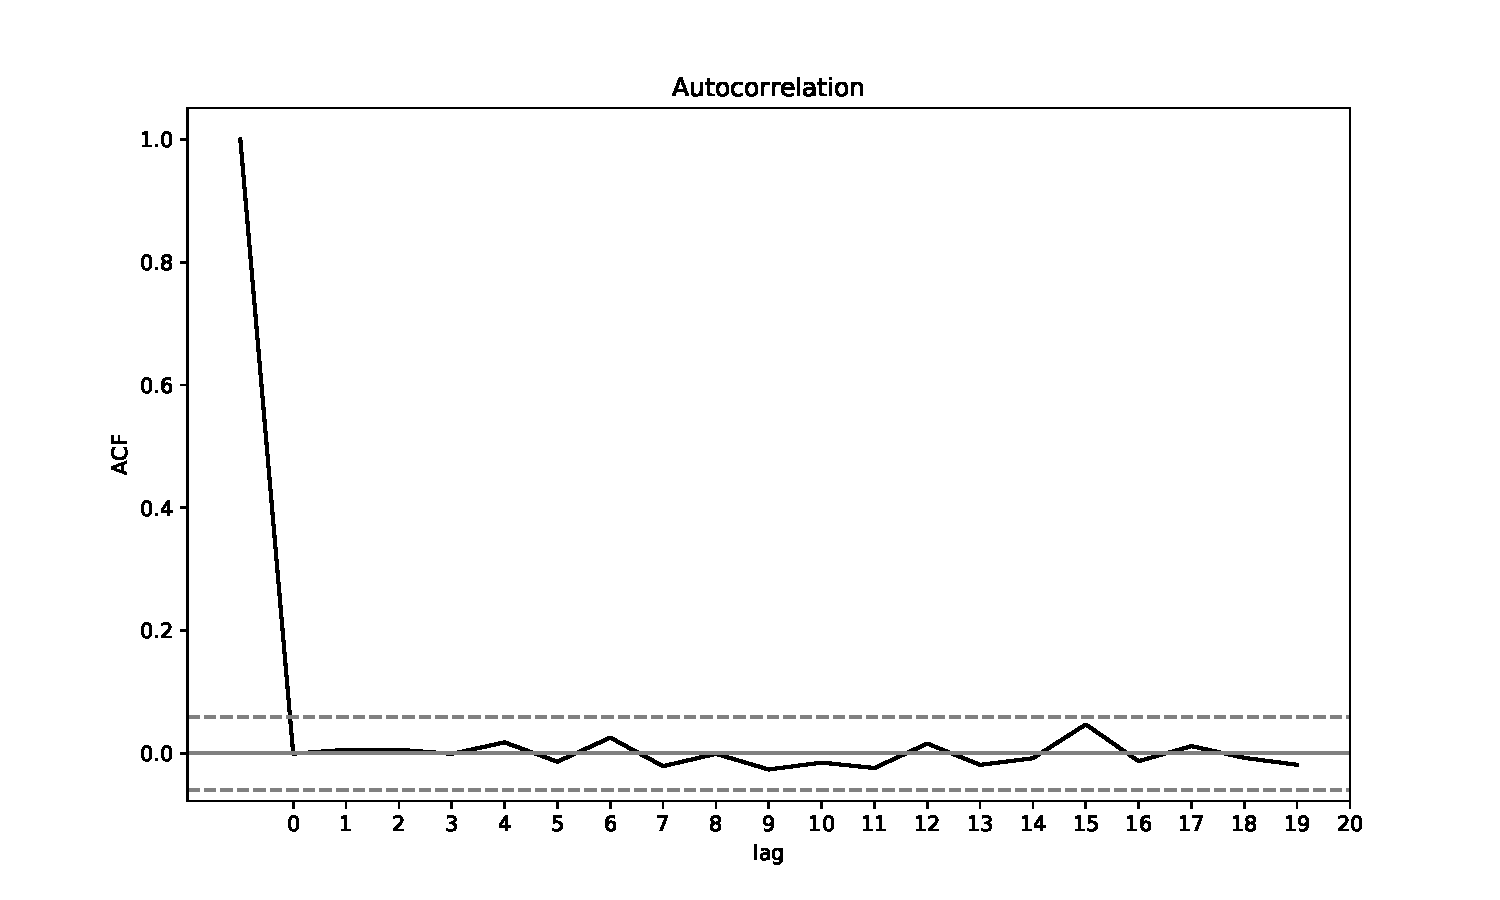
\includegraphics{../output/BE/plot/figACF_WN.pdf}

\end{comment}

\usepackage{fancyhdr} % This should be set AFTER setting up the page geometry
\pagestyle{fancy} % options: empty , plain , fancy
\renewcommand{\headrulewidth}{0pt} % customise the layout...
\lhead{}\chead{}\rhead{}
\lfoot{}\cfoot{\thepage}\rfoot{}

\renewenvironment{abstract}
{\list{}{\rightmargin\leftmargin}%
	\item[\textbf{\hspace{10mm}Abstract.}]\relax}
{\endlist}


%%% SECTION TITLE APPEARANCE
\usepackage{sectsty}
\allsectionsfont{\mdseries\upshape
	\sectionrule{15pt}{0pt}{-5pt}{1pt} }


\title{\textbf{Examination of a Demand Driven Real Estate Index Based on Search Query Data}}
\author{Jasmin Maag, 10-714-715}
\date{12 October 2018}
\begin{document}

%\clearpage
\maketitle
%\thispagestyle{fancy}

\begin{abstract}
%	\emph{
	An up-to-date index that is able to reflect the demand for real estate is needed not only in practice, but as well for theoretical applications. Based on Google search inquiries, indices for the search term ``Wohnung'' in the cantons Zurich and Bern are constructed. These indices are then approached with the classical decomposition model.
%}
\end{abstract}

\section*{Introduction}
Real estate is an indispensable good of an economy. Besides serving as a necessary living space for private individuals, construction and maintenance generate a large number of jobs. And as a financial asset---either as a private investment or grouped into real estate funds---it can create significant added value for the investor, and at the same time have the power to throw an entire economy into a crisis: real estate-bubble warnings are a recurring subject in the media all around the world. However, despite the importance of the real estate market, there is not a lot of information about the interplay of its supply and demand. For example, new investment projects are often justified by assessing demand for real estate based on retrospective measures such as past market transactions.
In the American real estate market, researchers have therefore begun to include search query data in order to improve the quality of pricing models. For example, \cite{wubrynjolffsson} show that the number of Google search inquiries for ``real estate agencies'' and ``real estate listings'' have a significant influence on the number of home sales and on house prices.
 \\
 In this short paper two demand-driven real estate indices for the cantons Zurich (ZH) and Bern (BE) are constructed based on Google search inquiries for the term ``Wohnung''. In a second step the indices are modeled with a classical decomposition approach.

\section{Data}
The website Google Trends allows users to analyze the popularity of specific search terms in a country and time period. The daily number of search inquiries for a time period is normalized to a percentage of the highest number in this time period. That is to say, the number of inquiries of the day with the highest number of inquiries in a time period is set to 100 and the number of the other days relative to that (\cite{googleT}). In this paper the daily number of search inquiries for the term ``Wohnung'' is used as a data basis. For this 1,098 daily files were downloaded, covering the time period 31 August 2015 to
31 August 2018. Since the daily number showed a lot of noise, the daily data was smoothed by taking a moving average of the previous 7 days. Hence, the final indices for the cantons ZH and BE cover the period 6 September 2015 to 31 August 2018. An overview of the two indices is shown in Figure \ref{fig:orig}. As can be seen, both indices show a slightly increasing trend over the three years under observation.

\begin{figure}[p!]
	\begin{minipage}{.5\linewidth}
		\centering
		\resizebox{1\linewidth}{!}{
			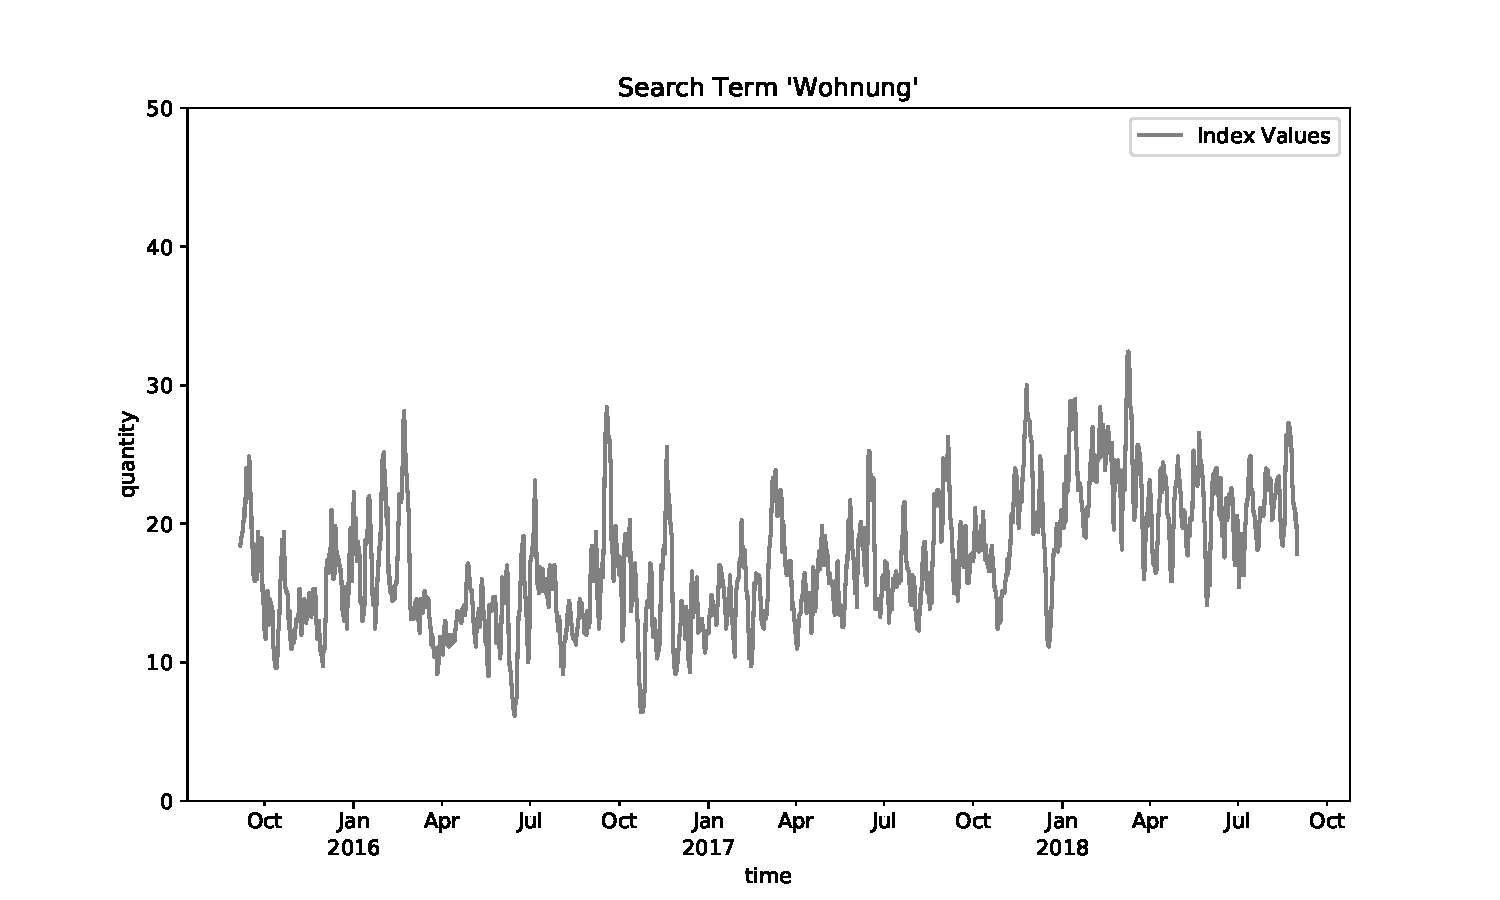
\includegraphics{../output/ZH/plot/figOrig.pdf}}
	\end{minipage}	\begin{minipage}{.5\linewidth}
		\centering
		\resizebox{1\linewidth}{!}{
			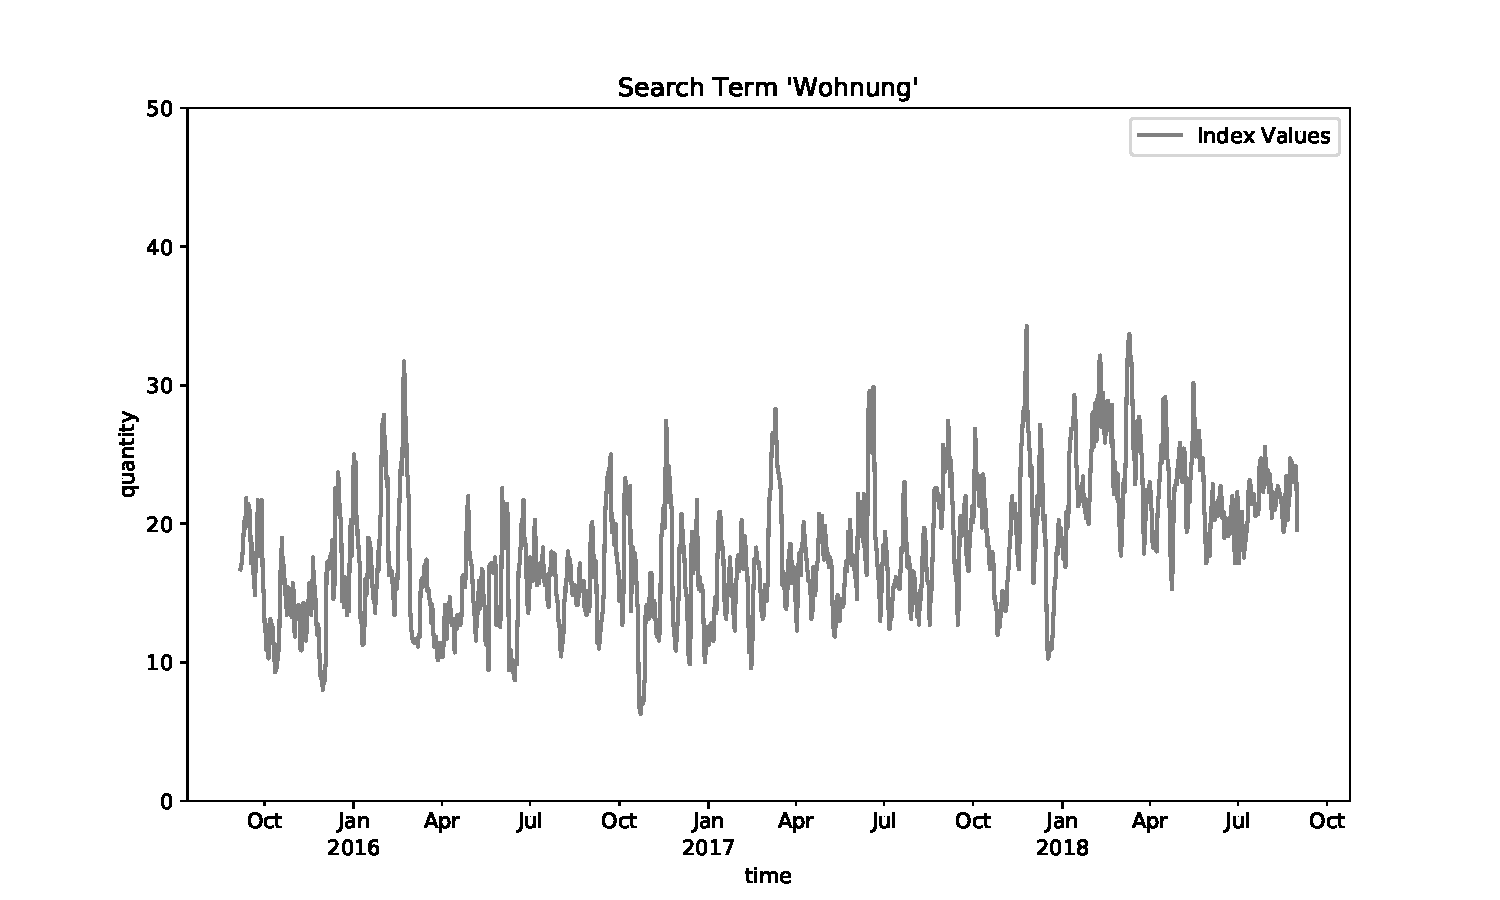
\includegraphics{../output/BE/plot/figOrig.pdf}}
	\end{minipage}
	\caption{Plots of the indices ZH (left) and BE (right). The x-axis describes the time from 6 September 2015 to 31 August 2018, and the y-axis the daily popularity of the search term ``Wohnung''. Source: own elaboration based on \cite{googleT}.}
	\label{fig:orig}
\end{figure}

\section{The Classical Decomposition Model}
The classical decomposition model is based on the idea that any non-stationary time series can be separated into non-stationary and stationary components. In this paper, an underlying additive model is assumed. Hence, the model is
\begin{equation}
 X_{t}=T_{t}+C_{t}+S_{t}+E_{t},
 \end{equation}
 where \(T_t\) describes the trend, \(C_t\) the cyclical component, \(S_t\) the season, and \(E_t\) the error component (\cite{brockdavTHEORY}). Regarding the two index series for ZH and BE, for \(T_t\) a linear trend model is chosen, for \(S_t\) a simple seasonal average, and \(E_t\) is modeled as an ARMA(\(p,q\)) process. Since the data covers only three years, \(C_t\) was assumed to be not present. The decomposition model was calculated for the period 6 September 2015 to 24 August 2018. The period 25 to 31 August 2018 was left out in order to forecast future values with the final models.

\section{Application}
In a first attempt a linear trend model is chosen for \(T_t\). In practical applications it is common to use a polynomial function up to order two (\cite{schlittAPPLIED}). Hence, three different polynomial functions \(m_t\) are fitted to the indices,
\begin{enumerate}
	\item \(m_t=\beta_1+\beta_2t\)
	\item \(m_t=\beta_1+\beta_3t^2\)
	\item \(m_t=\beta_1+\beta_2t+\beta_3t^2\)
\end{enumerate}
The models are fitted with a linear regression and the parameters are estimated with OLS. In line with \cite{schlittAPPLIED} the model with the lowest \(BIC\) is chosen to represent \(T_t\).
 For ZH the trend model \(x_t=\beta_1+\beta_2t+\beta_3t^2\) showed the lowest \(BIC\) with 5915.25, and for BE the model \(m_t=\beta_1+\beta_3t^2\) with a \(BIC\) of 6124.47.
 An overview of the modeled trend functions is given in Table \ref{tab:trend}. The parameters are significant on a 5 percent significance level. Further, a plot of the trend function alongside the index values is provided in Figure \ref{fig:trend}.
 \\
In order to model the season, the modeled trend values have to be subtracted from the original data. Figure \ref{fig:season} shows a yearly overview of the de-trended indices ZH and BE. Although the de-trended series show no obvious seasonality, \(S_t\) was calculated as a simple seasonal average in order to further reduce the noise in the data. A graphical overview of the de-trended and de-seasonalized indices is given in Figure \ref{fig:error}. As can be seen, the data no longer shows any significant deviation from stationarity, and the error term is ready to be modeled.
\begin{table}[p]
	\centering
	\begin{minipage}{1\linewidth}
		\centering
		\import{"../output/ZH/table/"}{"trend_table.tex"}
		\vspace*{0.7 cm}
	\end{minipage}
	\begin{minipage}{1\linewidth}
		\centering
		\import{"../output/BE/table/"}{"trend_table.tex"}
		\vspace*{0.7 cm}
	\end{minipage}
	\caption{Overview of the fitted polynomial trend functions for the indices ZH (top) and BE (bottom). Source: own elaboration based on \cite{googleT}.}
	\label{tab:trend}
\end{table}
\begin{figure}[p!]
	\begin{minipage}{.5\linewidth}
		\centering
		\resizebox{1\linewidth}{!}{
			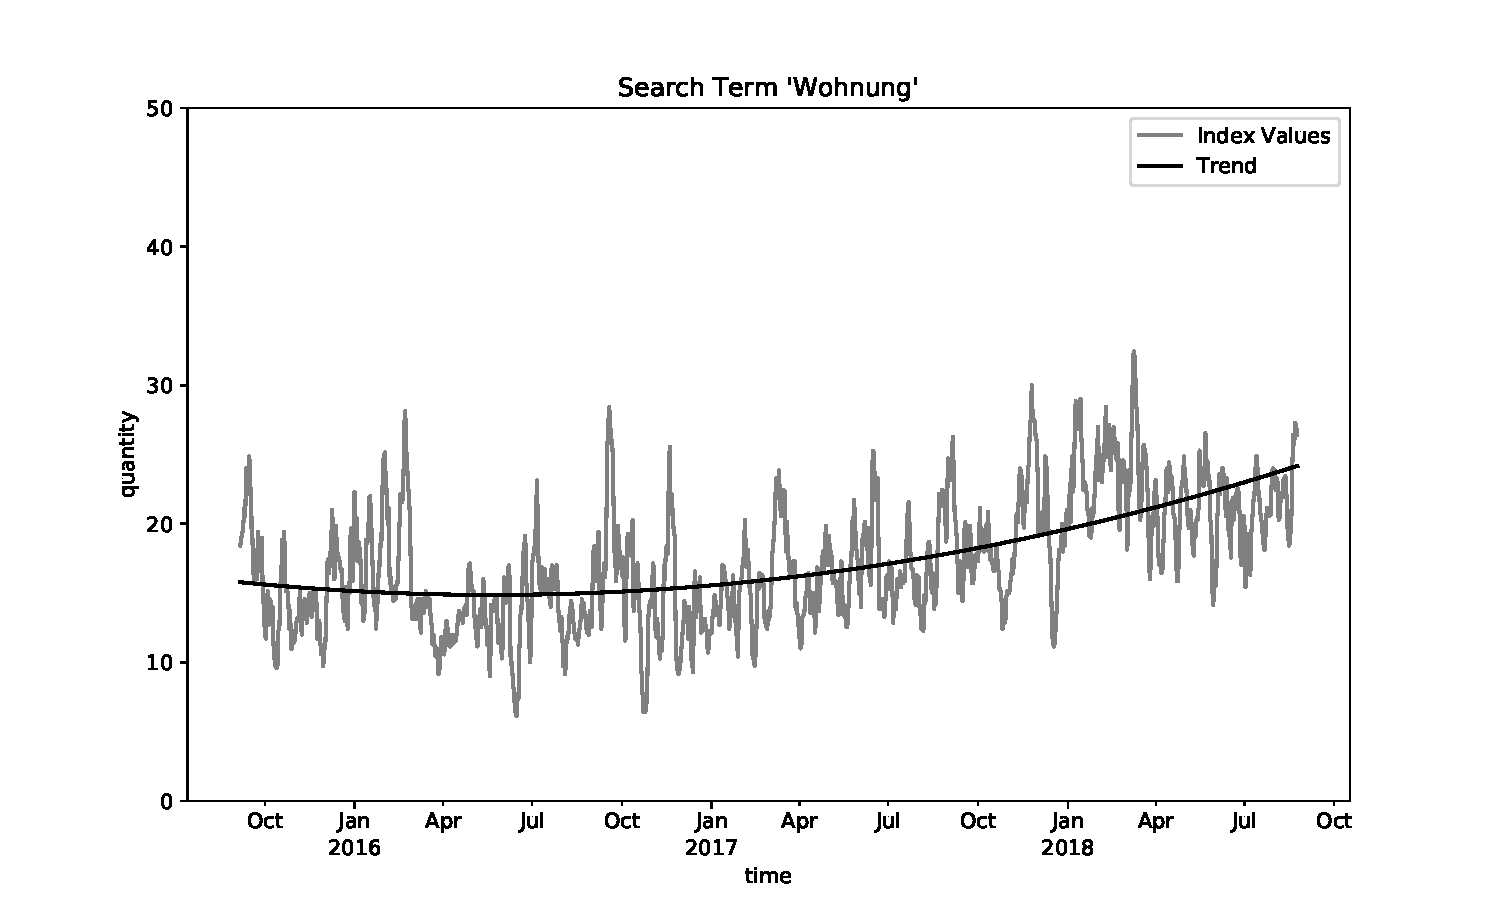
\includegraphics{../output/ZH/plot/figTrend.pdf}}
	\end{minipage}	\begin{minipage}{.5\linewidth}
		\centering
		\resizebox{1\linewidth}{!}{
			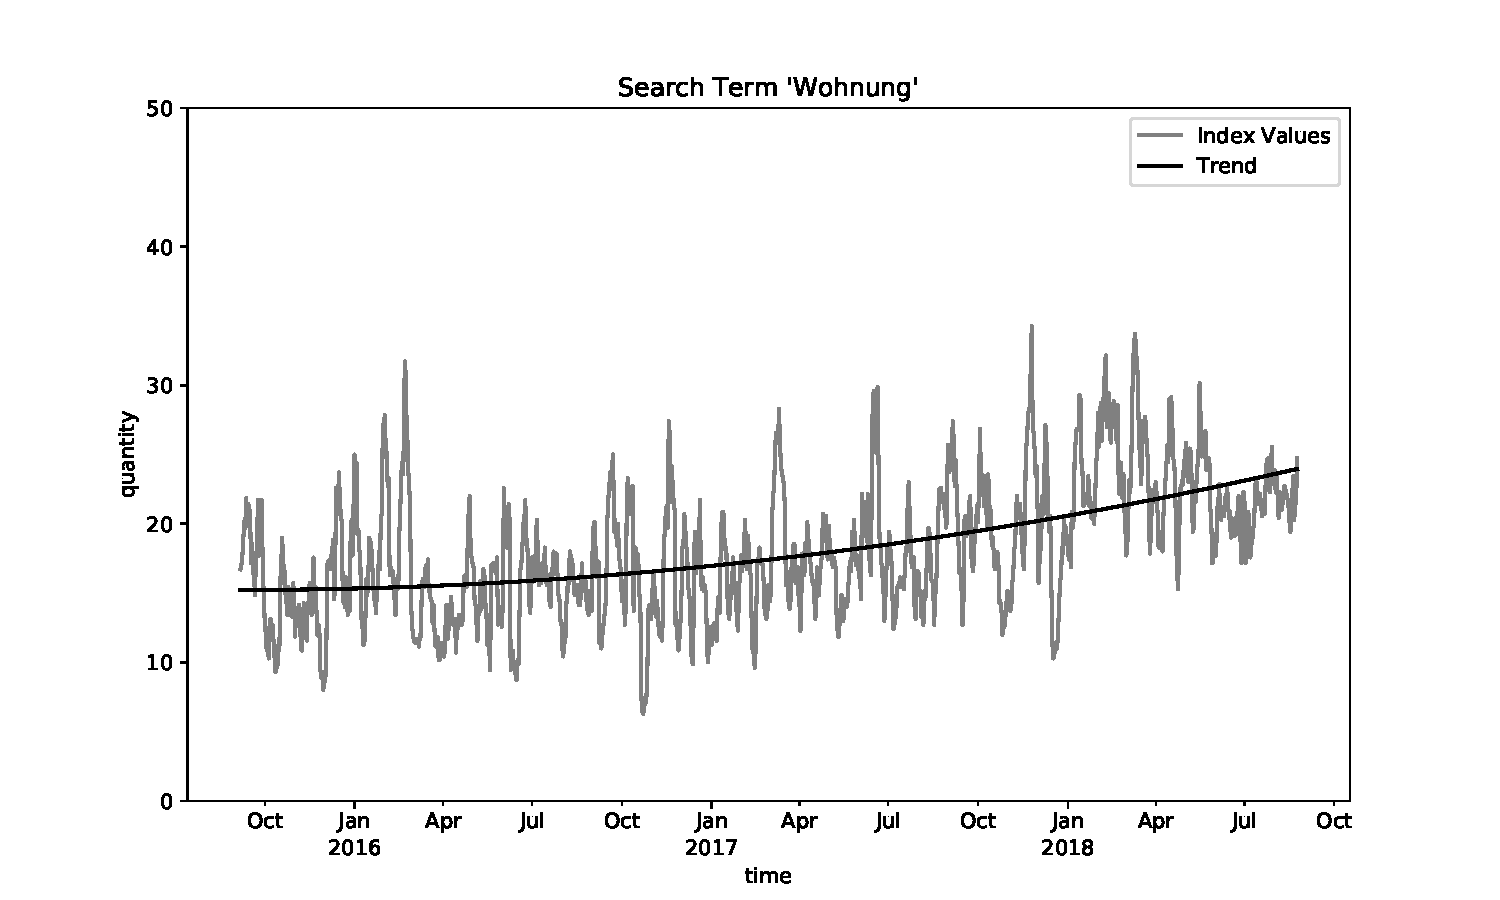
\includegraphics{../output/BE/plot/figTrend.pdf}}
	\end{minipage}
	\caption{Plots of the indices ZH (left) and BE (right) with their polynomial trend functions. The x-axis describes the time from 6 September 2015 to 24 August 2018, and the y-axis the daily popularity of the search term ``Wohnung''. Source: own elaboration based on \cite{googleT}.}
	\label{fig:trend}
\end{figure}
\begin{figure}[p!]
	\begin{minipage}{.5\linewidth}
		\centering
		\resizebox{1\linewidth}{!}{
			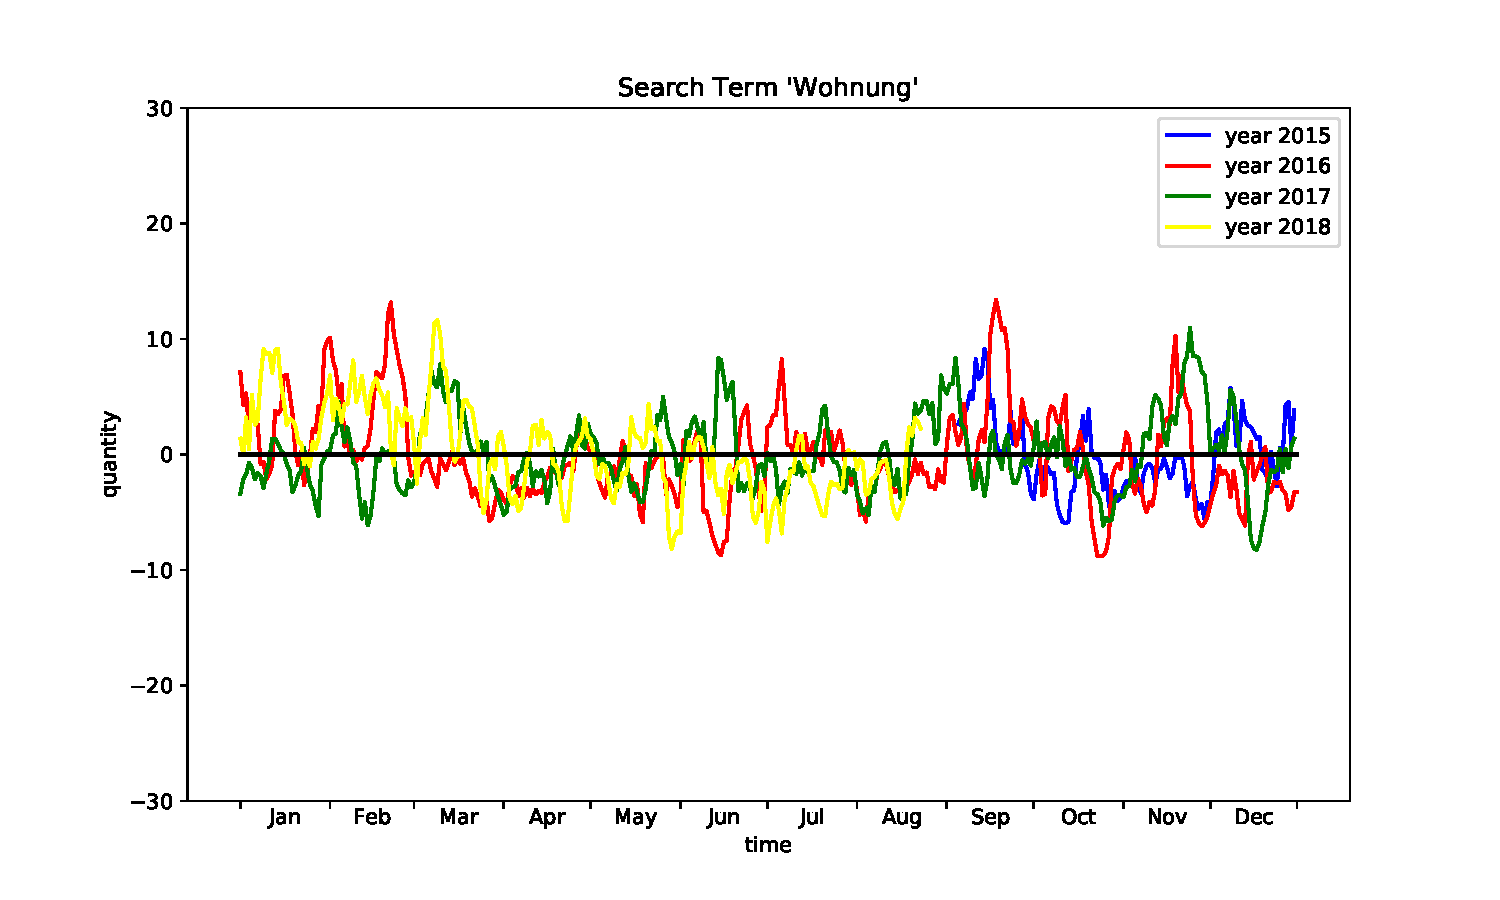
\includegraphics{../output/ZH/plot/figSeason.pdf}}
	\end{minipage}	\begin{minipage}{.5\linewidth}
		\centering
		\resizebox{1\linewidth}{!}{
			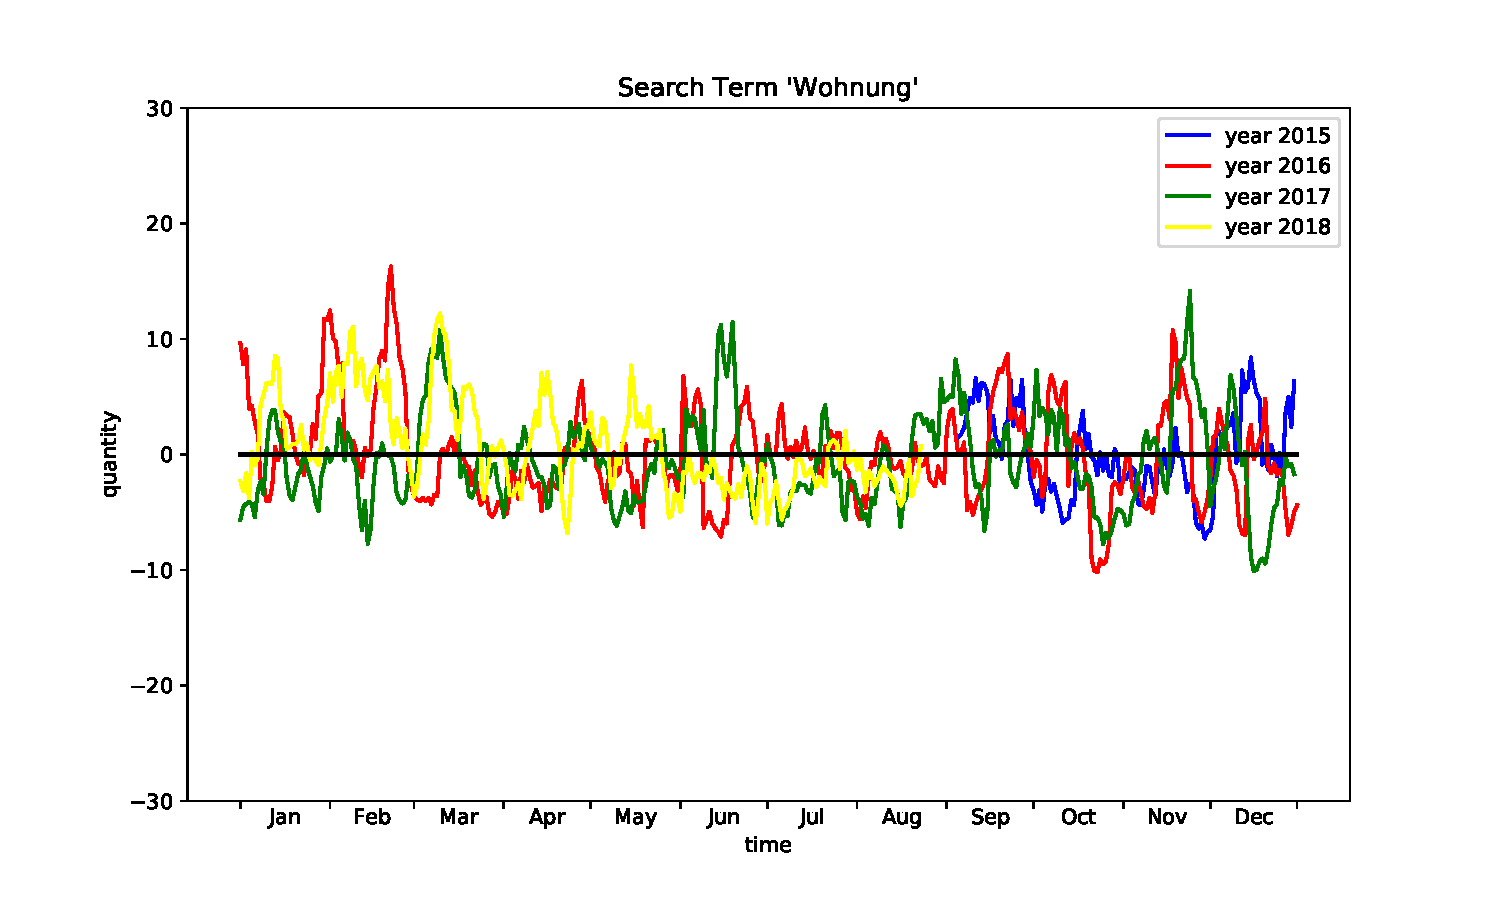
\includegraphics{../output/BE/plot/figSeason.pdf}}
	\end{minipage}
	\caption{Seasonal overview of the de-trended indices ZH (left) and BE (right) for the years 2015-2018. The x-axis describes the days in a year, and the y-axis the daily popularity of the search term ``Wohnung''. Source: own elaboration based on \cite{googleT}.}
	\label{fig:season}
\end{figure}
\begin{figure}[p!]
	\begin{minipage}{.5\linewidth}
		\centering
		\resizebox{1\linewidth}{!}{
			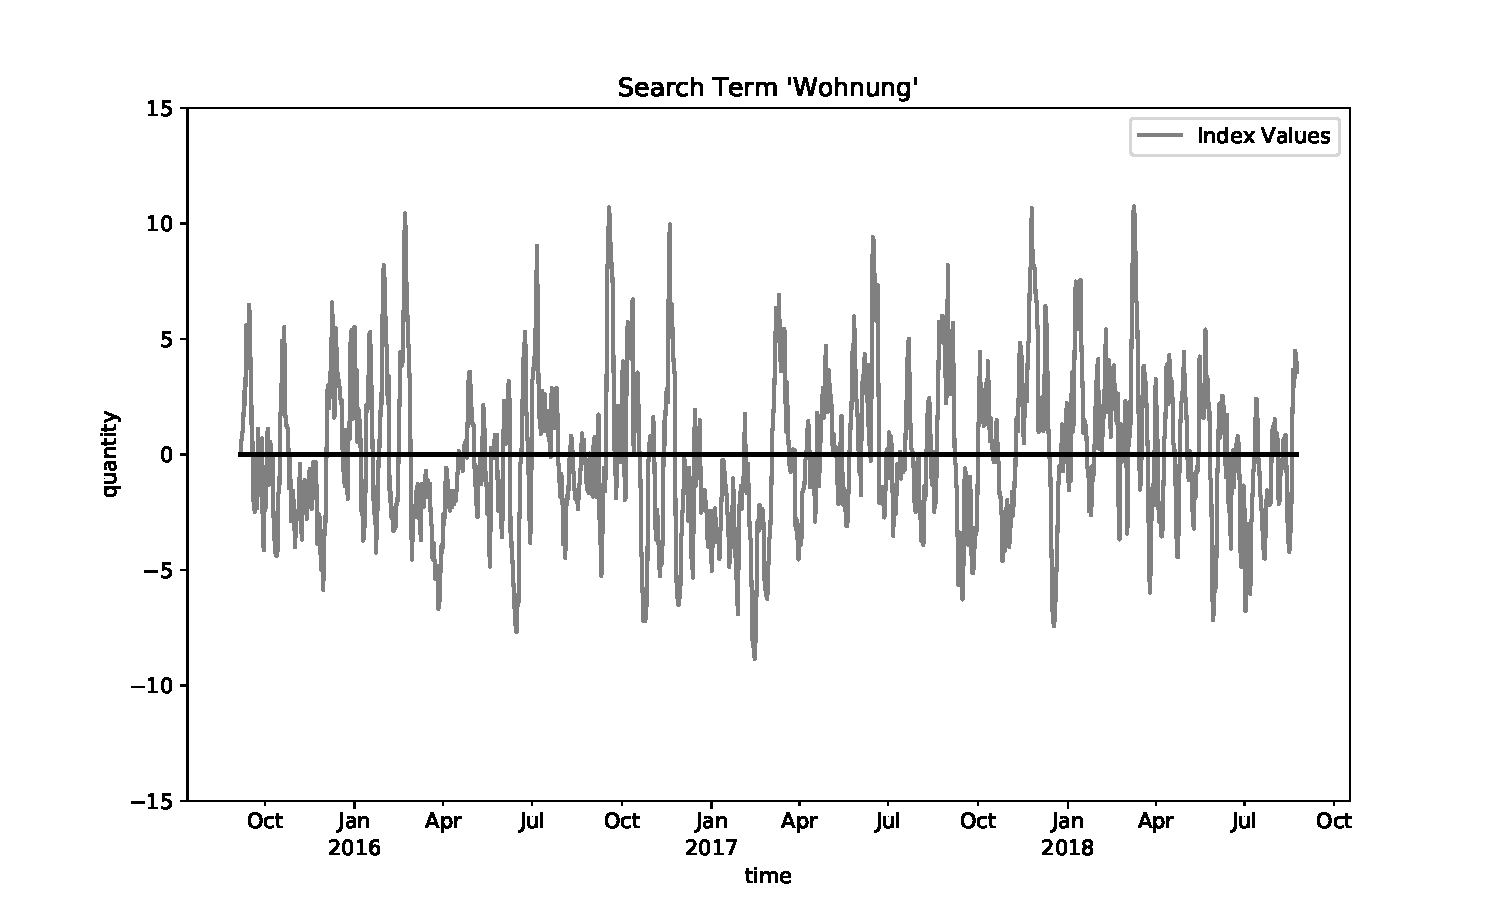
\includegraphics{../output/ZH/plot/figError.pdf}}
	\end{minipage}	\begin{minipage}{.5\linewidth}
		\centering
		\resizebox{1\linewidth}{!}{
			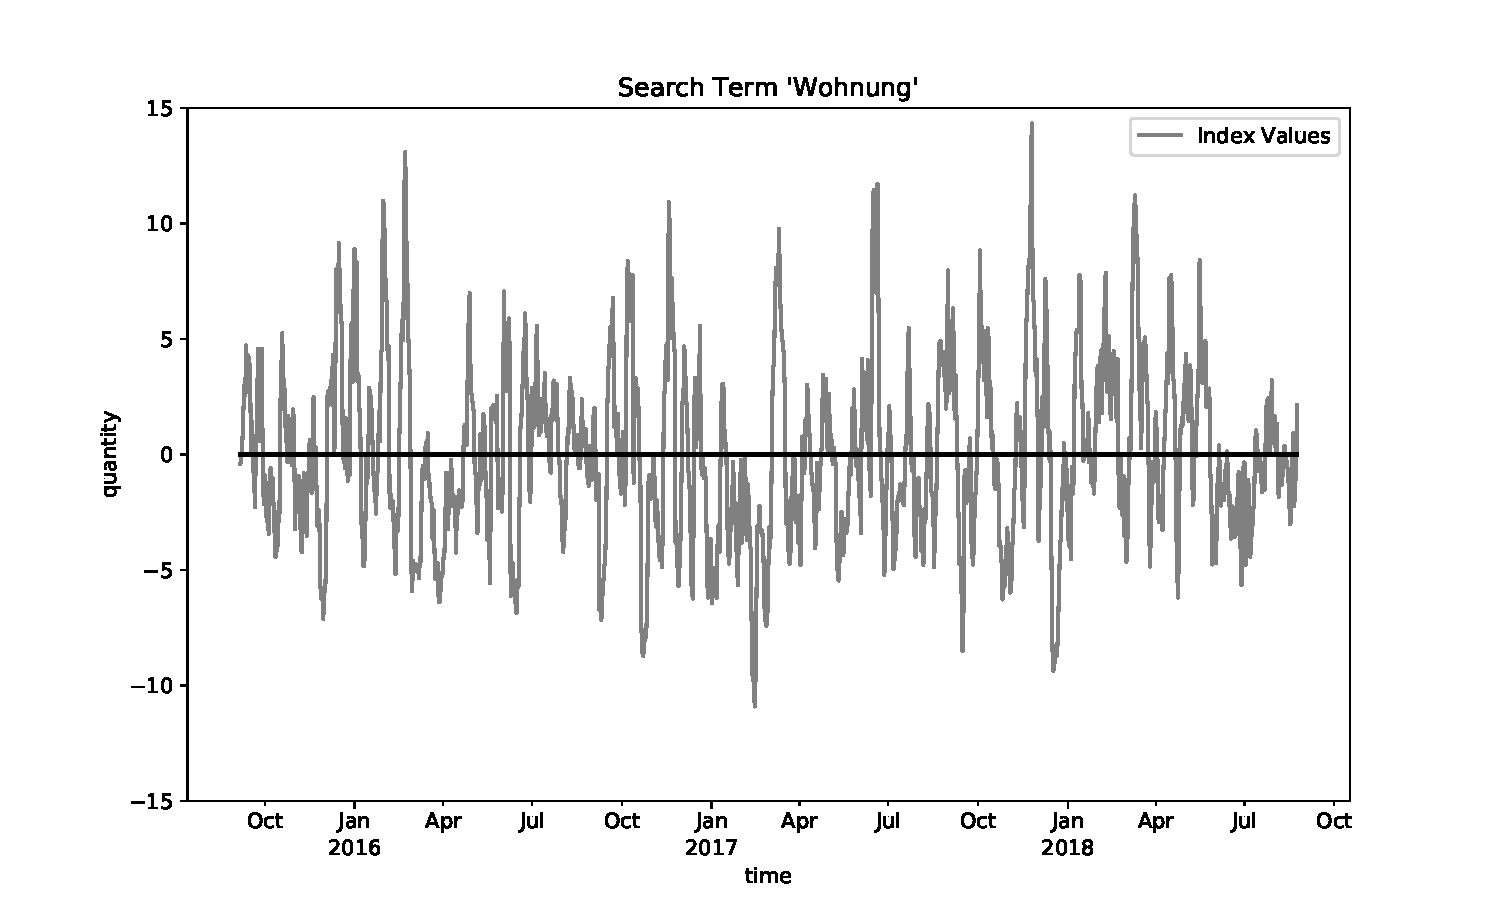
\includegraphics{../output/BE/plot/figError.pdf}}
	\end{minipage}
	\caption{Plots of the de-trended and de-seasonalized indices ZH (left) and BE (right). The x-axis describes the time from 6 September 2015 to 24 August 2018, and the y-axis the daily popularity of the search term ``Wohnung''. Source: own elaboration based on \cite{googleT}.}
	\label{fig:error}
\end{figure}

As mentioned in the beginning, \(E_t\) is approached with an ARMA(\(p,q\)) model. To find the best combination of the orders \(p\) and \(q\), the dependency structure of the error series is assessed by plotting the autocorrelation function (ACF), partial autocorrelation function (PACF), and by calculating the vector-correlations. Mathematically the vector-correlation for orders \(p\) and \(q\) is defined as
\begin{equation}
\lambda(p,q)=(-1)^p\cdot\frac{\kappa_{p+1,q+1}}{\kappa_{p+1,0}},
\label{eq:vectorcorrelation}
\end{equation}
where \(\kappa_{p,q}\) describes the determinant of a Toeplitz matrix with the ACF value \(\rho(q)\) as main diagonal element (\cite{schlittTHEORY}).
The vector correlations should take on values equal or close to 0 for combinations of \(p\) and \(q\), where \(p\) and \(q\) are equal to or higher than the real orders \(p\) and \(q\) of the underlying ARMA(\(p,q\)) process (\cite{schlittTHEORY}).
The vector-correlations for combinations of \(p\leq6\) and \(q\leq6\) are given in Table \ref{tab:vectorcorr}. As can be seen, both vector-correlation tables show a ``zero'' block starting at \(p=3\) and \(q=2\). This would suggest a \(p\) and \(q\) combination of 3 and 2 for both indices. However, the ACF and PACF plots in Figures \ref{fig:ACFPACF_ZH} and \ref{fig:ACFPACF_BE} show significant values up to lag 6, and 14 respectively. Thus, to find the best combination of \(p\) and \(q\), the corrected Akaike information criterion (\(AICc\)) is calculated. The \(AICc\) is defined as
\begin{equation}
 AICc=AIC+\frac{2(p+q)(p+q+1)}{n-p-q-1},
\end{equation}
where \(AIC\) is the normal Akaike information criterion and \(n\) the number of observations. An overview of the \(AICc\) values for combinations of \(p\leq7\) and \(q\leq7\) is given in Table \ref{tab:aicc}. For both indices the lowest values are found for \(p=1\) and \(q=6\). Hence, for ZH and BE an ARMA(\(1,6\)) is modeled to the error series. An overview of the found ARMA(\(1,6\)) is given in Table \ref{tab:error}. Based on a 5 percent significance level, both error models show significant parameters.
\\
In order to asses the error model's fit, the residuals of the error model should be inspected for randomness, and if they show any remaining dependency structure. For this, the ACF and PACF values of the residuals are plotted in the Figures \ref{fig:ACFPACFWN_ZH} and \ref{fig:ACFPACFWN_BE}. Neither the ACF nor the PACF plots overstep the 95 percent boundaries. In conclusion, the fitted ARMA(\(1,6\)) model for the error component of the indices ZH and BE provides a good fit.
\begin{table}[p]
	\centering
	\begin{minipage}{1\linewidth}
		\centering
		\import{"../output/ZH/table/"}{"vectorcorr_df.tex"}
		\vspace*{0.7 cm}
	\end{minipage}
	\begin{minipage}{1\linewidth}
		\centering
		\import{"../output/BE/table/"}{"vectorcorr_df.tex"}
		\vspace*{0.7 cm}
	\end{minipage}
	\caption{Vector-correlation tables for the error series of the indices ZH (top) and BE (bottom). Source: own elaboration based on \cite{googleT}.}
	\label{tab:vectorcorr}
\end{table}
\begin{figure}[p!]
	\begin{minipage}{.5\linewidth}
		\centering
		\resizebox{1\linewidth}{!}{
			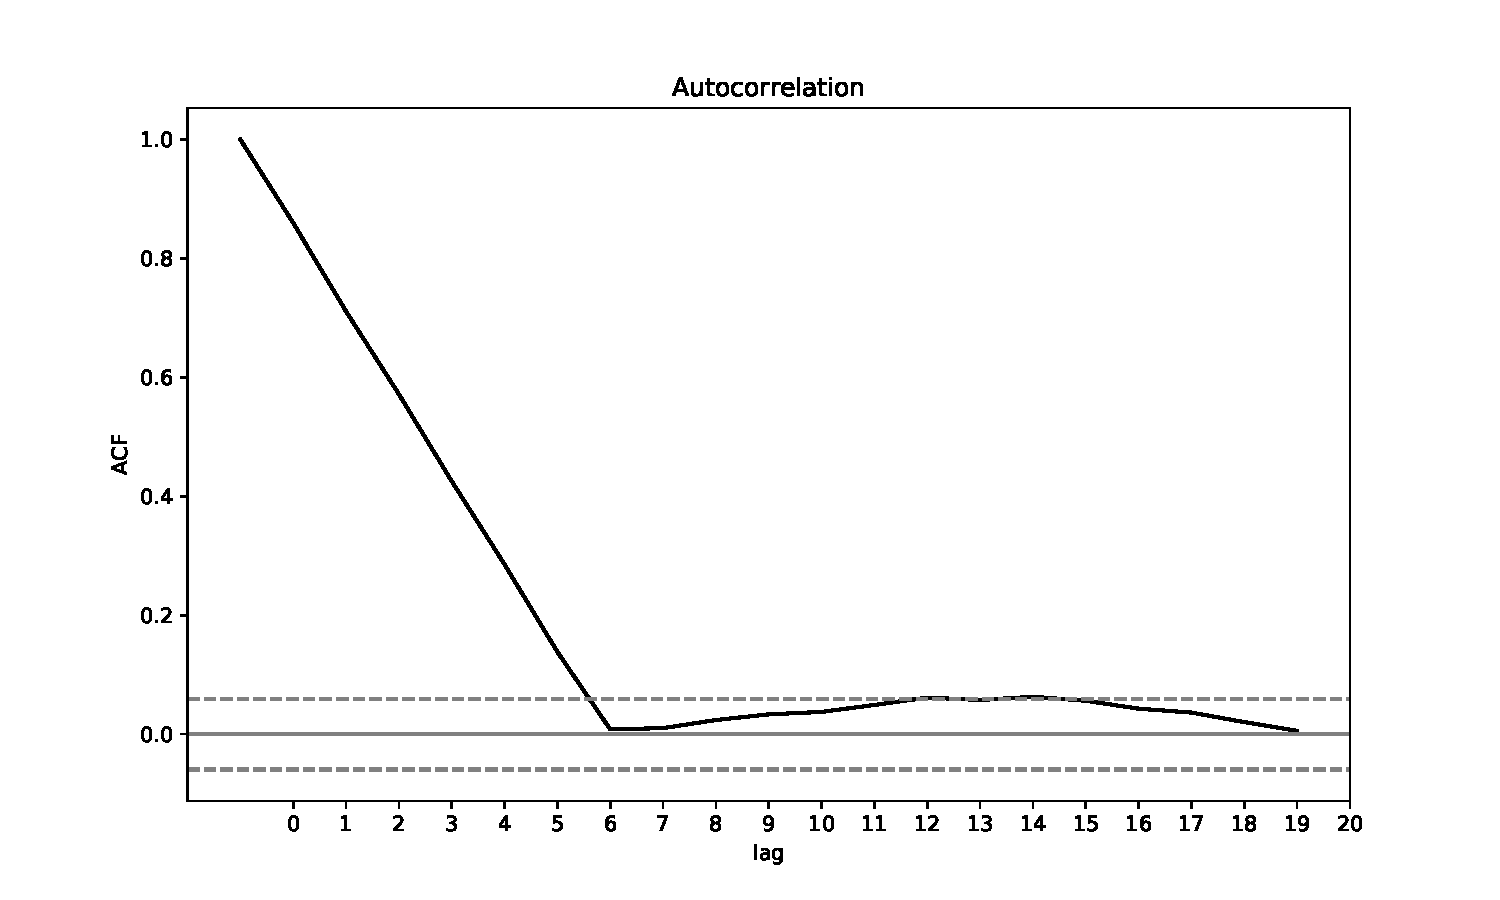
\includegraphics{../output/ZH/plot/figACF.pdf}}
	\end{minipage}	\begin{minipage}{.5\linewidth}
		\centering
		\resizebox{1\linewidth}{!}{
			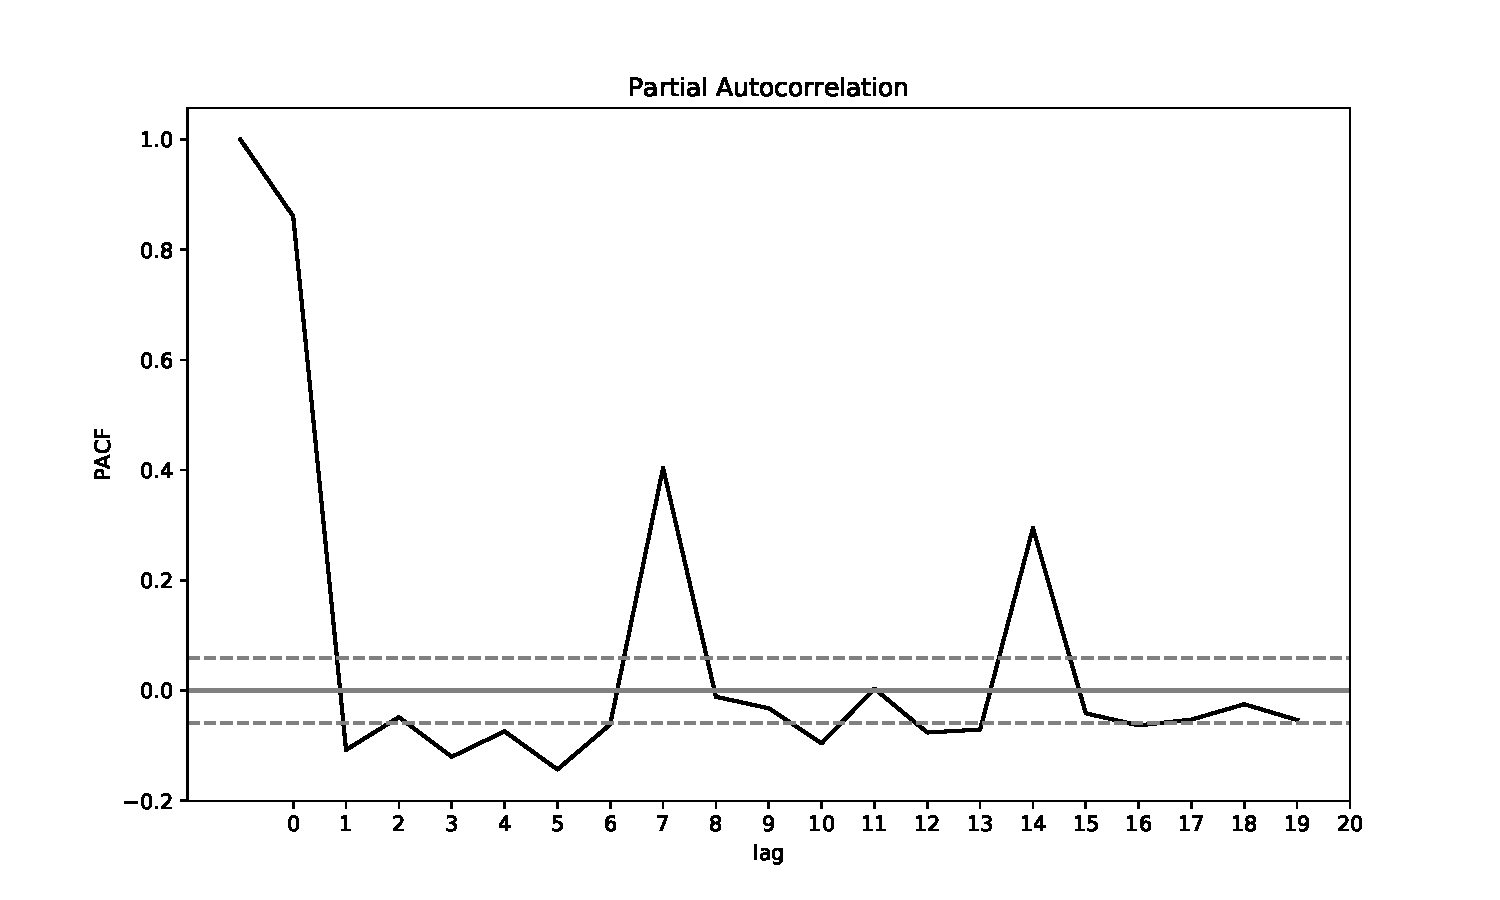
\includegraphics{../output/ZH/plot/figPACF.pdf}}
	\end{minipage}
	\caption{ACF and PACF plots of the de-trended and de-seasonalized index ZH. The x-axis describes the lag, and the y-axis the function value. Source: own elaboration based on \cite{googleT}.}
	\label{fig:ACFPACF_ZH}
\end{figure}
\begin{figure}[p!]
	\begin{minipage}{.5\linewidth}
		\centering
		\resizebox{1\linewidth}{!}{
			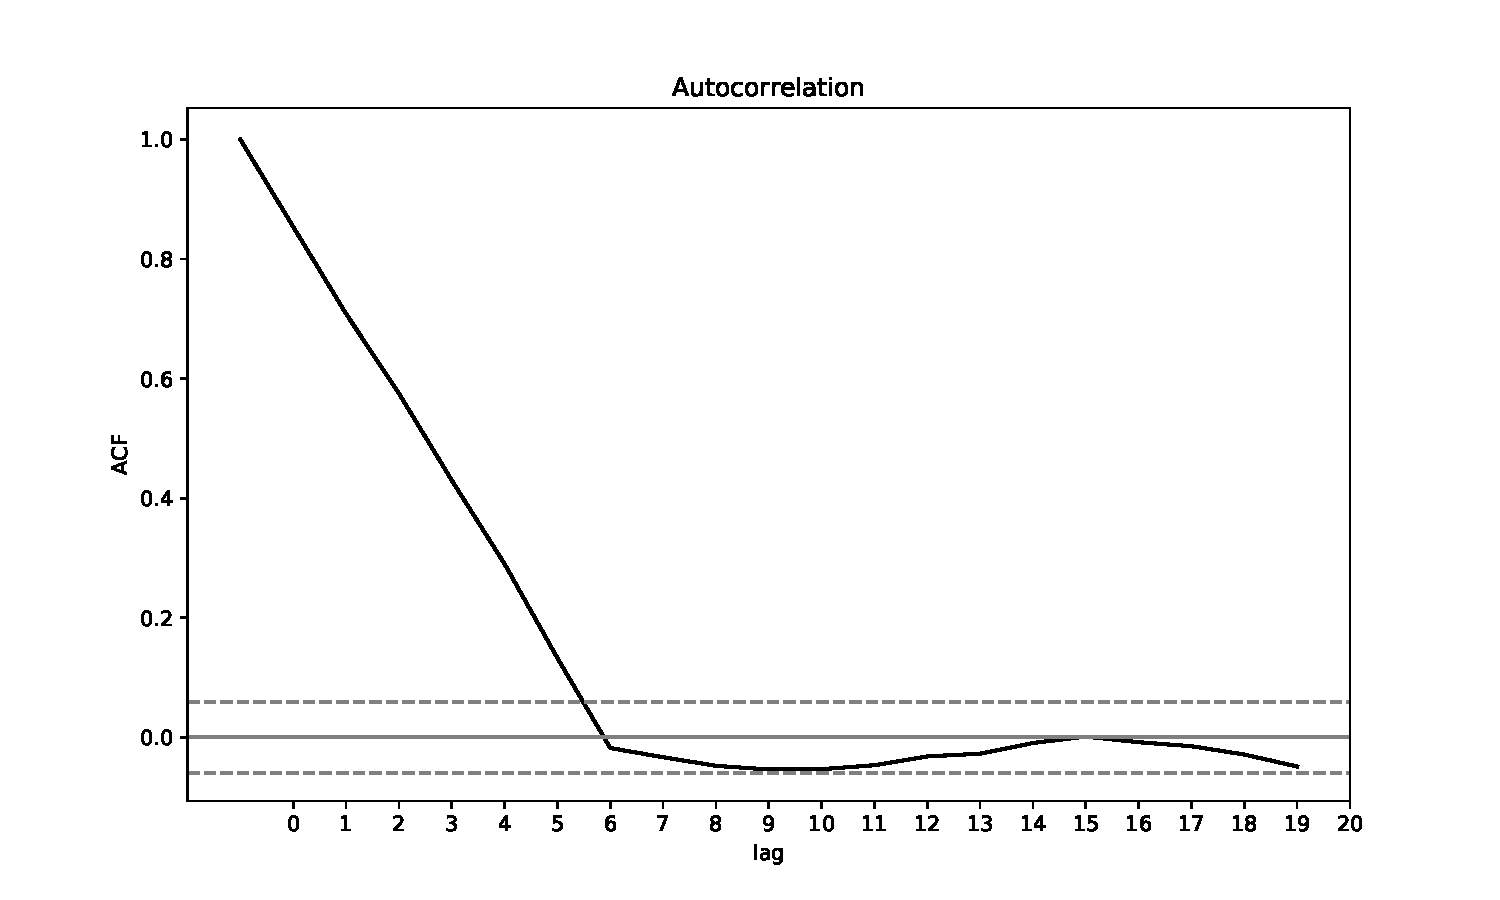
\includegraphics{../output/BE/plot/figACF.pdf}}
	\end{minipage}	\begin{minipage}{.5\linewidth}
		\centering
		\resizebox{1\linewidth}{!}{
			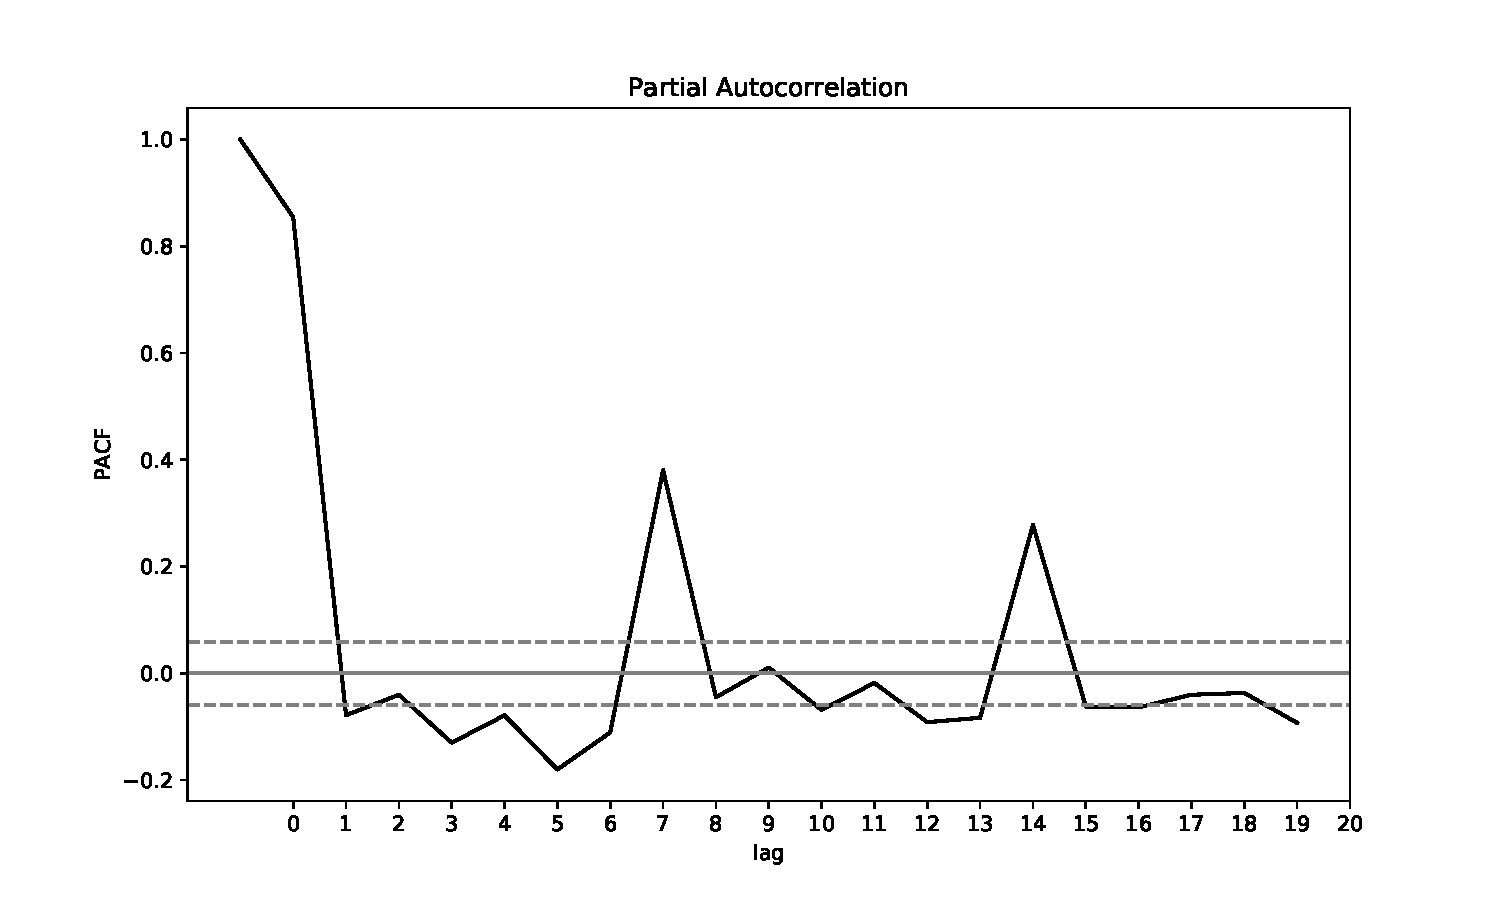
\includegraphics{../output/BE/plot/figPACF.pdf}}
	\end{minipage}
	\caption{ACF and PACF plots of the de-trended and de-seasonalized index BE. The x-axis describes the lag, and the y-axis the function value. Source: own elaboration based on \cite{googleT}.}
	\label{fig:ACFPACF_BE}
\end{figure}
\begin{table}[p]
	\centering
	\begin{minipage}{1\linewidth}
		\centering
		\import{"../output/ZH/table/"}{"aicc_df.tex"}
		\vspace*{0.7 cm}
	\end{minipage}
	\begin{minipage}{1\linewidth}
		\centering
		\import{"../output/BE/table/"}{"aicc_df.tex"}
		\vspace*{0.7 cm}
	\end{minipage}
	\caption{\(AICc\) tables for the error series of the indices ZH (top) and BE (bottom). Source: own elaboration based on \cite{googleT}.}
	\label{tab:aicc}
\end{table}
\begin{table}[p]
	\centering
	\begin{minipage}{1\linewidth}
		\centering
		\import{"../output/ZH/table/"}{"error_table.tex"}
		\vspace*{0.7 cm}
	\end{minipage}
	\begin{minipage}{1\linewidth}
		\centering
		\import{"../output/BE/table/"}{"error_table.tex"}
		\vspace*{0.7 cm}
	\end{minipage}
	\caption{Overview of the fitted error models for the indices ZH (top) and BE (bottom). Source: own elaboration based on \cite{googleT}.}
	\label{tab:error}
\end{table}
\begin{figure}[p!]
	\begin{minipage}{.5\linewidth}
		\centering
		\resizebox{1\linewidth}{!}{
			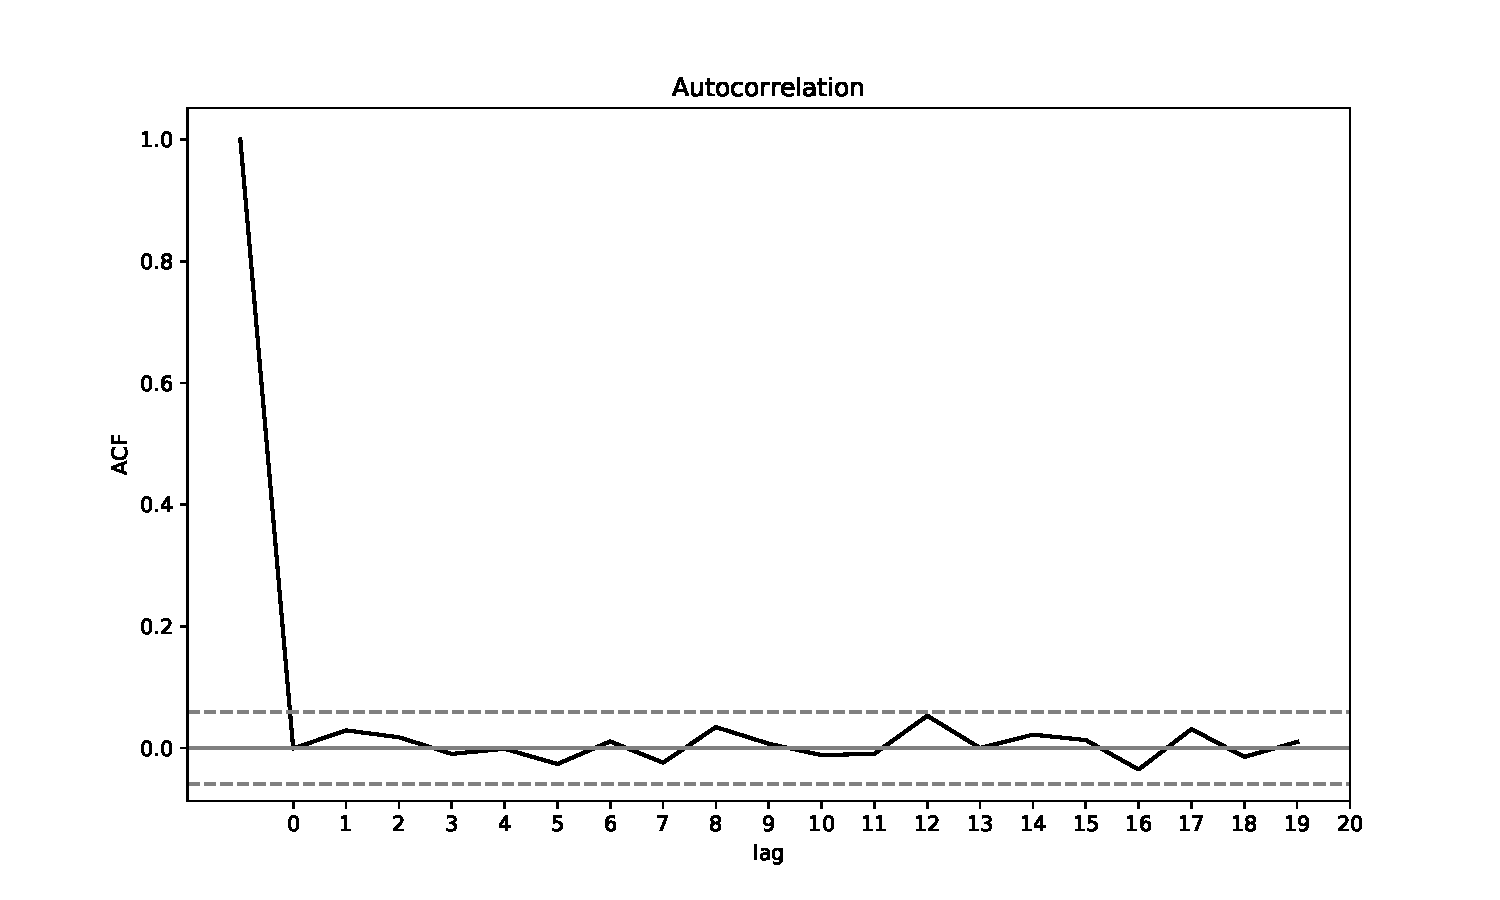
\includegraphics{../output/ZH/plot/figACF_WN.pdf}}
	\end{minipage}	\begin{minipage}{.5\linewidth}
		\centering
		\resizebox{1\linewidth}{!}{
			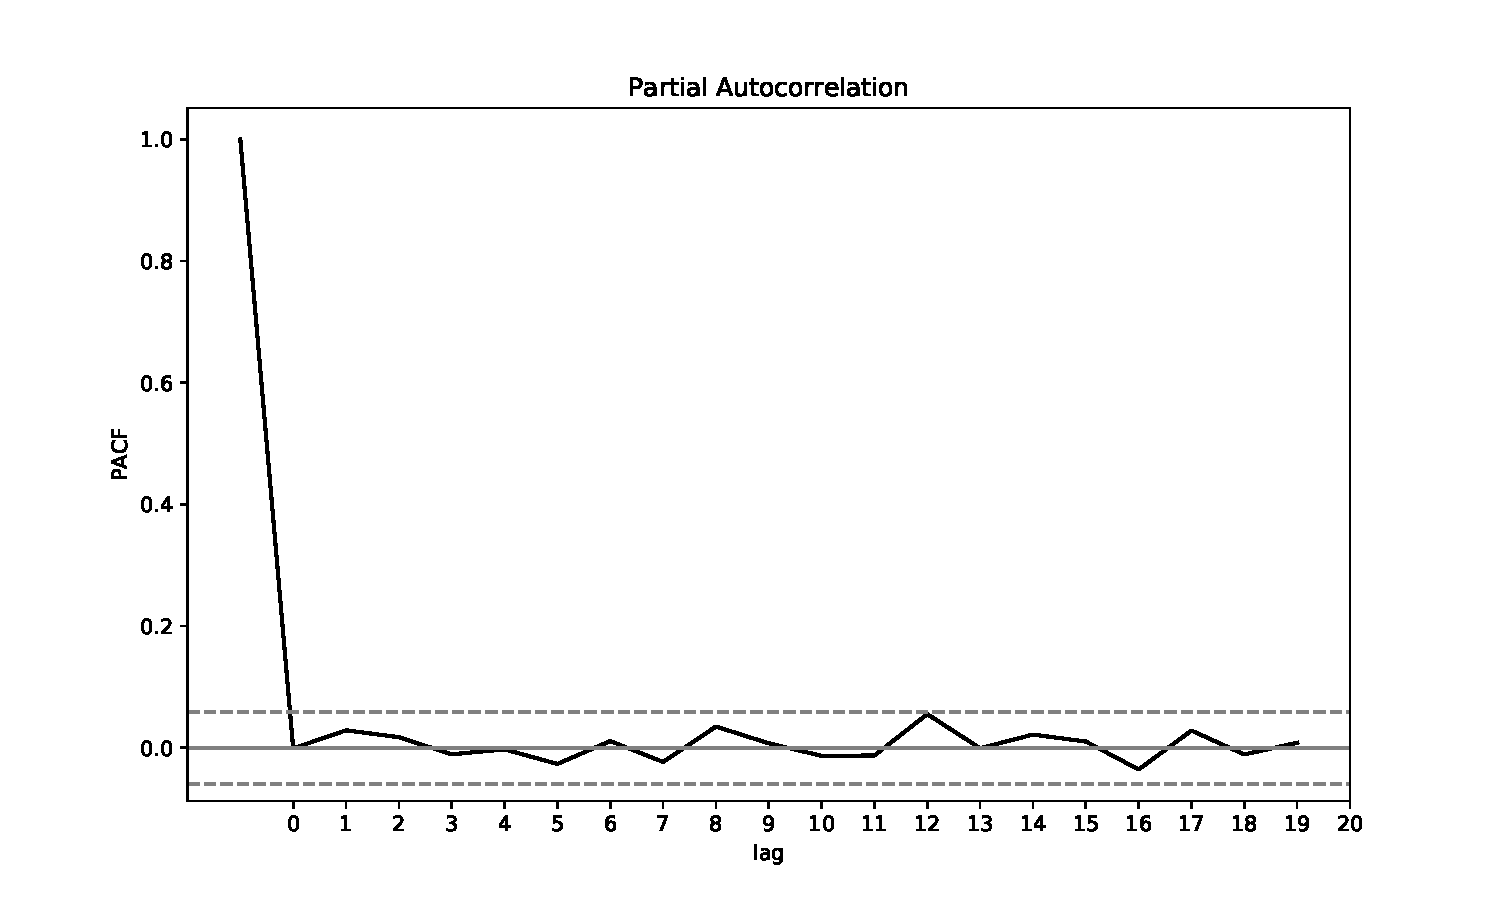
\includegraphics{../output/ZH/plot/figPACF_WN.pdf}}
	\end{minipage}
	\caption{ACF and PACF plots of the error residuals of the index ZH. The x-axis describes the lag, and the y-axis the function value. Source: own elaboration based on \cite{googleT}.}
	\label{fig:ACFPACFWN_ZH}
\end{figure}
\begin{figure}[p!]
	\begin{minipage}{.5\linewidth}
		\centering
		\resizebox{1\linewidth}{!}{
			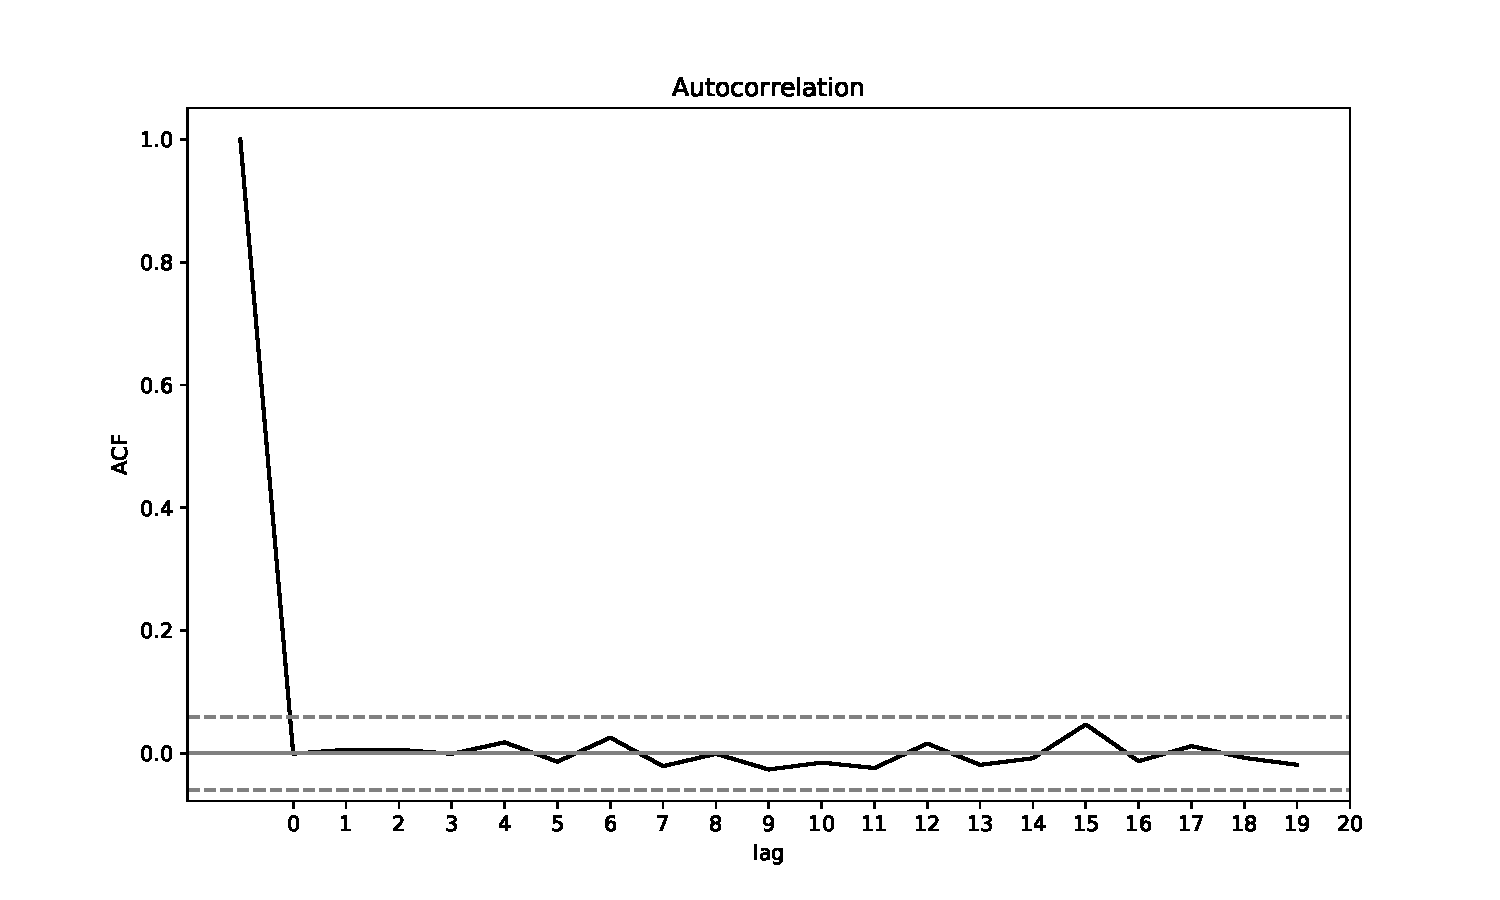
\includegraphics{../output/BE/plot/figACF_WN.pdf}}
	\end{minipage}	\begin{minipage}{.5\linewidth}
		\centering
		\resizebox{1\linewidth}{!}{
			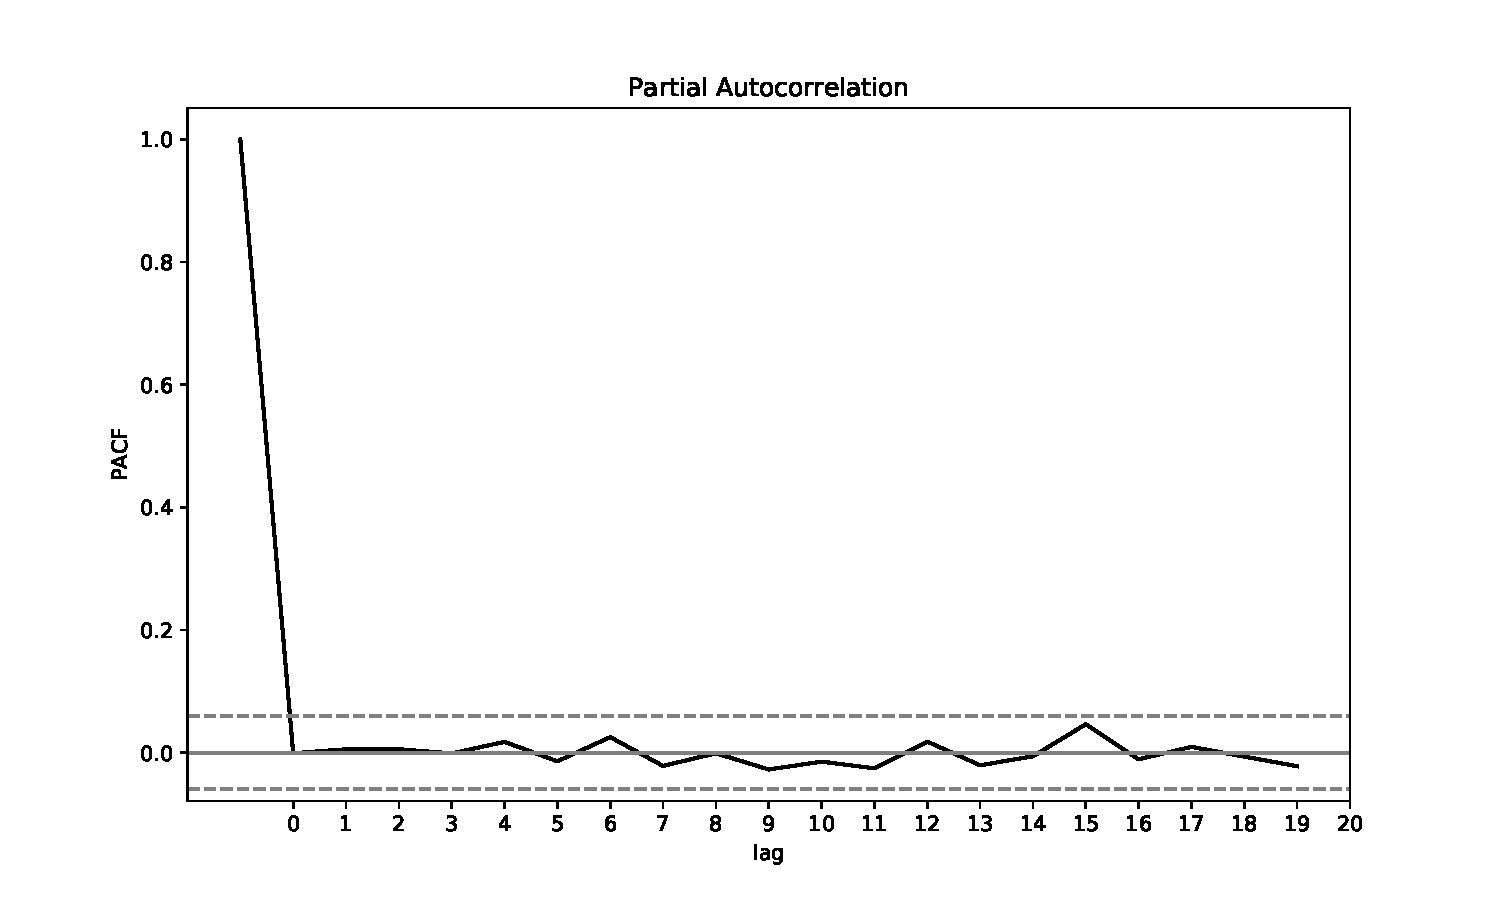
\includegraphics{../output/BE/plot/figPACF_WN.pdf}}
	\end{minipage}
	\caption{ACF and PACF plots of the error residuals of the index BE. The x-axis describes the lag, and the y-axis the function value. Source: own elaboration based on \cite{googleT}.}
	\label{fig:ACFPACFWN_BE}
\end{figure}

In a final step the overall fit of the calculated decomposition model is assessed. To do so, the mean absolute percentage error (\(MAPE\)) for the in- and out-of-sample period was calculated. The general \(MAPE\) formula is
\begin{equation}
	MAPE=\frac{100}{n}\sum_{t=1}^{n} \left|\frac{x_t-\hat{x}_t}{x_t}\right|,
\end{equation}
where \({x_t}\) are the observed values, and \(\hat{x}_t\) the model's estimated values for a time period of length \(n\). For both indices the in-sample \(MAPE\)s are fairly low with approximately 0.006. The out-of sample \(MAPE\) is 1.24 for ZH and 0.69 for BE. Additionally, the original values are plotted alongside the modeled values in Figure \ref{fig:finalModel}. The modeled values seem to fit pretty closely to the original values.
\begin{figure}[h]
	\begin{minipage}{1\linewidth}
		\centering
		\resizebox{1\linewidth}{!}{
			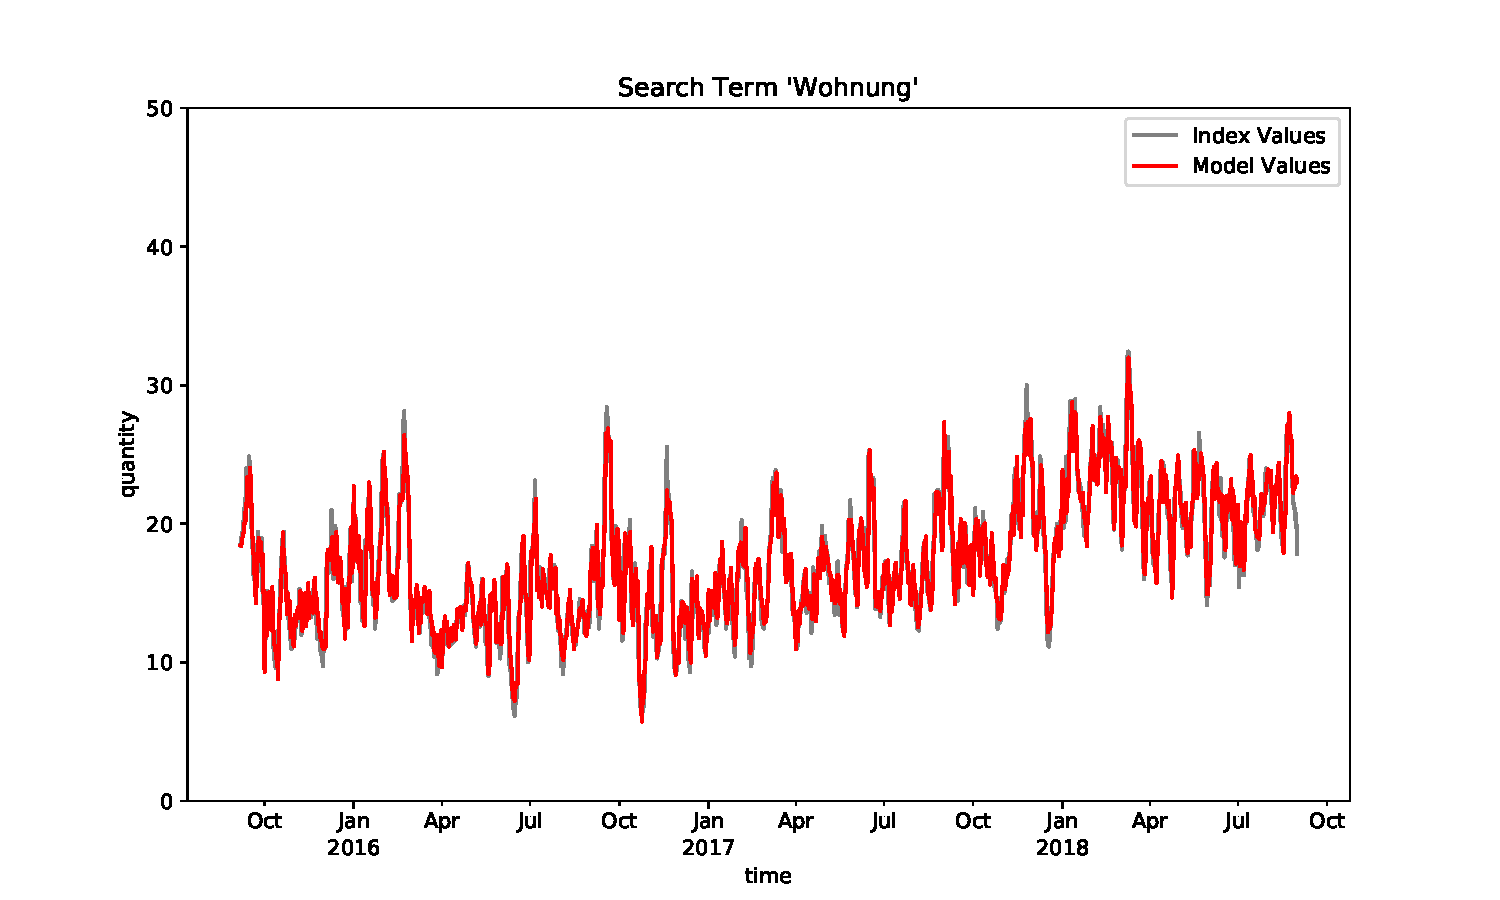
\includegraphics{../output/ZH/plot/figModel.pdf}}
	\end{minipage}	\begin{minipage}{1\linewidth}
		\centering
		\resizebox{1\linewidth}{!}{
			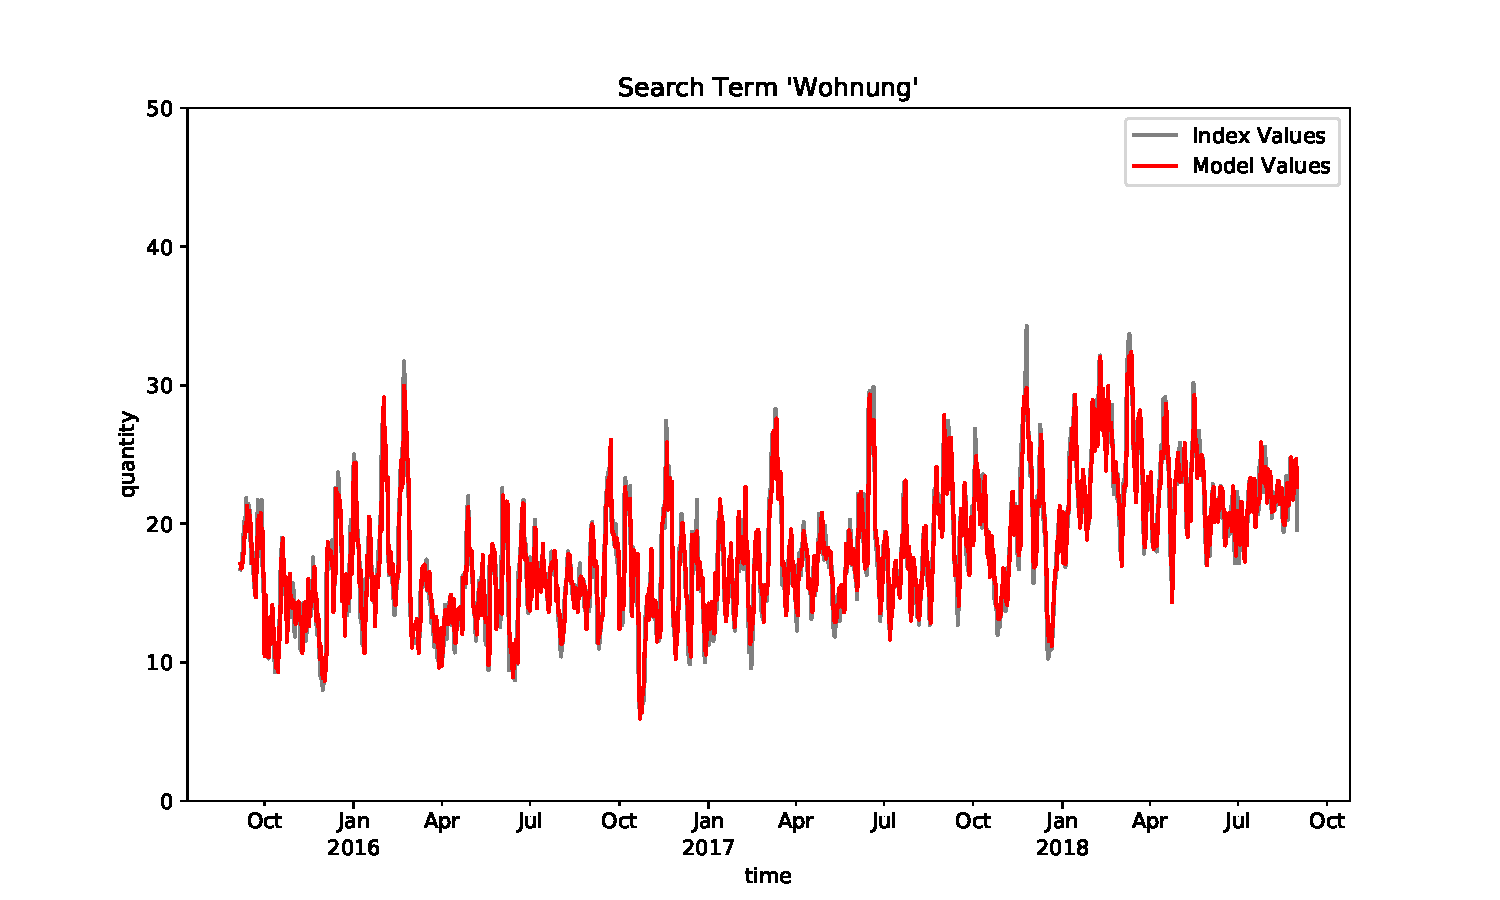
\includegraphics{../output/BE/plot/figModel.pdf}}
	\end{minipage}
	\caption{Plots of the indices ZH (top) and BE (bottom) with their decomposition model functions. The x-axis describes the time from 6 September 2015 to 31 August 2018, and the y-axis the daily popularity of the search term ``Wohnung''. Source: own elaboration based on \cite{googleT}.}
	\label{fig:finalModel}
\end{figure}

\section*{Conclusion}
The task of this paper was to construct an up-to-date index for the demand for real estate. Based on Google search inquiries for the term ``Wohnung'' two indices for the cantons Zurich and Bern were constructed and modeled with a decomposition approach.
Overall, the modeled components of the decomposition model showed fairly good results with parameter \(p\)-values far below a 5 percent significance level. However, it is questionable if it was indeed necessary to calculate a seasonal component, since a season did not show to be prominently present in the yearly overview of the de-trended indices. Further, the close fit of the modeled values to the original values suggests that overfitting might be present. Improving the modeled indices and investigating the problem of overfitting will be left to future research.
\begin{comment}
\import{"../output/BE/table/"}{"aicc_df.tex"}
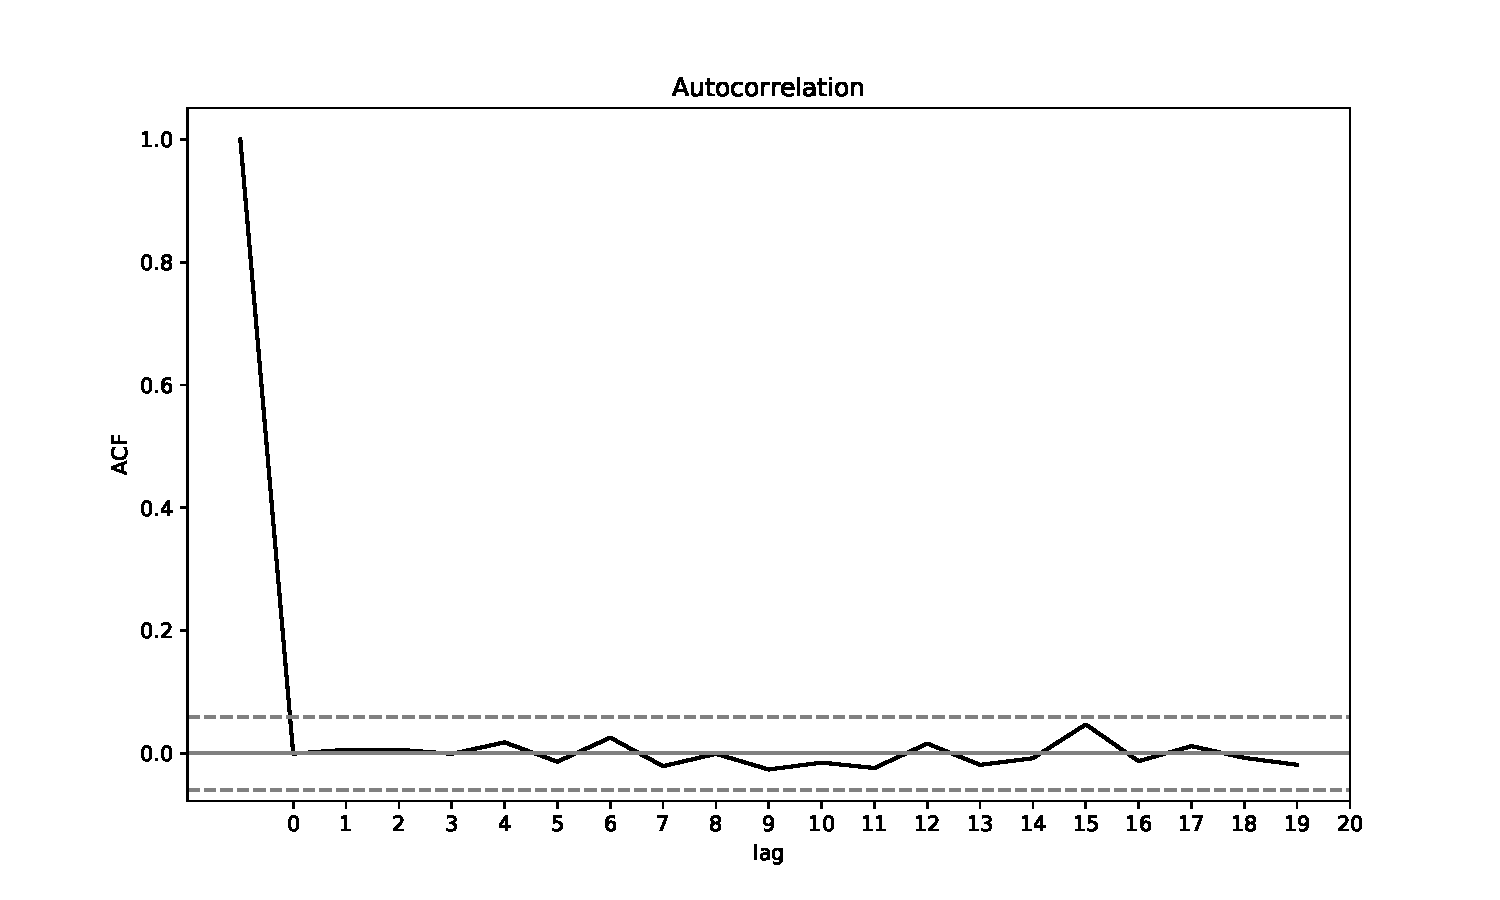
\includegraphics{../output/BE/plot/figACF_WN.pdf}
\end{comment}







\newpage
\clearpage
\singlespacing
\bibliography{bibiDoc.bib}









\end{document}
